\documentclass{kththesis}

\usepackage{blindtext} % This is just to get some nonsense text in this template, can be safely removed

\usepackage{csquotes} % Recommended by biblatex
\usepackage[style=numeric,sorting=none,backend=biber]{biblatex}
\addbibresource{references.bib} % The file containing our references, in BibTeX format

\usepackage{pgfplotstable,filecontents}
\pgfplotsset{compat=1.9}% supress warning
\usepackage{booktabs,colortbl}


\title{Determining Important Features for Melanoma Classification Through Feature Selection}
\alttitle{Värdering av attribut för klassificering av hudcancer}
\author{Vilmer Jonsson \\ Tor Strimbold}
\supervisor{Kevin Smith}
\examiner{Pawel Herman} 
\programme{Bachelor's Degree in Computer Science}
\school{School of Electrical Engineering and Computer Science}
\date{\today}

% Uncomment the next line to include cover generated at https://intra.kth.se/kth-cover?l=en
\kthcover{kth-cover.pdf} % Cover page background file, placeholder for now


\begin{document}

% Frontmatter includes the titlepage, abstracts and table-of-contents
\frontmatter

\titlepage

\begin{abstract}
  Skin cancer is a common disease in both Sweden and the United States. Although common, the survival rate of melanoma patients is high if the diagnosis is made at an early stage. Computer aided diagnostics has been shown to have potential in accurately diagnosing the disease utilizing machine learning. Thus, machine learning algorithms can be used to effectively classify a skin lesions as either benign or malignant. These algorithms can be made more accurate and efficient by applying feature selection since it decreases the dimensionality of the feature space. The aim of this study is to apply feature selection on four different classifiers to compare morphological and SIFT features in order to determine which features are important for classifying melanoma.
  
  The results show that morphological features in general increased the accuracy more than the SIFT features, although it varied between different classifiers. Furthermore, forward selection was more effective than backward selection in terms of accuracy for two of the classifiers. Lastly, certain features were more effective than others, the most effective feature was "Solidity".
\end{abstract}


\begin{otherlanguage}{swedish}
  \begin{abstract}
    Hudcancer är en vanligt förekommande sjukdom i både Sverige och USA. Dock är sannolikheten att en patient kan botas från sjukdomen hög om diagnosen sker i ett tidigt stadium. Datordriven diagnostisering har visat sig kunna diagnostisera sjukdomen på ett effektivt och med hög säkerhet genom att tillämpa maskininlärning. På så vis kan maskininlärningsalgoritmer användas för att klassificera hudutslag som godartade eller inte. Dessa algoritmer kan effektiviseras genom att utföra attributurvalsmetoder då det minskar antalet dimensioner som behöver beräknas. Syftet med denna studie är att undersöka vilka attribut som är viktiga för klassificeringen. Detta gjordes genom att tillämpa attributurvalsmetoderna Sekventiell Framåt- och Bakåtselektion på fyra olika maskininlärningsalgoritmer med indata i form av morfologiska och SIFT-attribut.
    
    Resultaten visar att morfologiska attribut generellt föredrogs i större utsträckning än SIFT-attribut, detta varierade dock mellan olika klassificeringsmodeller. Vidare var Framåtselektion mer effektiv än bakåtselektion sett till träffsäkerhet för två av klassificeringsmodellerna. Slutligen var vissa attribut mer effektiva än andra, det mest effektiva attributet var "Soliditet".
  \end{abstract}
\end{otherlanguage}


\tableofcontents


% Mainmatter is where the actual contents of the thesis goes
\mainmatter


% TODO: Fix the references
\chapter{Introduction}
The frequency of malignant melanoma has in the last decade been on the rise in Sweden with approximately 60 000 people being diagnosed with the disease yearly. \parencite{sverige-hudcancer}.
A similar trend has been observed in the United States where the number of people diagnosed with the disease has doubled during the period 1982-2011 \parencite{aad-skin-cancer}.

% TODO: Fix the references, could not find the source in Drive
Skin cancer, although common, has a 5-year survival rate of 99\% if discovered at an early stage \parencite{skincancer_org_2019}.
This fact makes the diagnosis of malignant melanoma an essential part of the treatment of the disease. In the light of diagnosis, machine learning has become a subject of interest in many medical fields, dermatology included. Multiple studies have been conducted to evaluate the potential of the algorithms’ accuracy and applicability through so-called computer aided diagnostics (CAD). Concerning malignant melanoma, some studies have reached an accuracy of up to 90\% which competes with the experts in the field. % TODO: Här kan vi behöva en källa

The accuracy of machine learning algorithms is however heavily reliant on the feature extraction methods used, where relevant features in an image are extracted and then used in the classification of the skin lesion. An effective feature extraction in turn relies on determining which features to use. Which is the subject of feature selection where different features are compared in terms of their effect on the diagnostic accuracy. It has been shown that effective feature selection make classifiers more effective, accurate and cost-effective. \parencite{KarabulutEsraMahsereci2012Acso}

\section{Research Question}
In our thesis we studied the effect of two different feature selection methods upon 169 features and using 4 different machine learning models. We aim to answer: % Tempus är ksk fucked
\begin{enumerate}
    \item Which features are the most important in terms of classification accuracy?
    \item Is there a difference between different models concerning which features are most effective?
    \item Is there a difference between selection methods in terms of performance enhancement?
\end{enumerate}

\section{Approach}

To study the proposed research questions two different selection methods were used, namely Forward and Backwards Selection. To further widen the base for comparison four different machine learning models will be used: K-Nearest Neighbors, a one-layered Neural Network, Random Forest and Support Vector Machine. These models are widely used in the research of automatic skin lesion diagnosis which makes them relevant to study. % Källa

Two types of features were examined, morphological and SIFT features. The morphological features consisted primarily of so-called ABCD features but also of features calculated using different morphological formulas. The ABCD features are based on the clinical practice where a skin lesion is classified based on its asymmetry, border irregularity, color and diameter. The ABCD method is widely used when diagnosing skin lesions using machine learning due to its effectiveness and simplicity to implement. \parencite{JAIN2015735} % Lite väl mycket 'reklam'.
% Kanske skriva lite om SIFT
% typ: SIFT features are common occuring in image analysis and were added to the study since ABCD features have been sifted.

\section{Scope}

The study is limited by the number of features, selection methods and models being used.

Firstly the models are limited by the fact that they consist of only shallow machine learning models. An extension of the study could include a deep learning model such as a convoluted neural network.

Secondly, the study is limited by the feature selection methods being used where only feature selection by wrapper methods are used through the sequential backward and forward selection. Other methods such as filter methods and embedded methods could be used to find synergies between features and widen the scope of the study.

Thirdly, the features were only of two types. Including for example deep features would give further insight into how the different types of features affect the accuracy of the classifiers.

\chapter{Background}

\section{Skin Cancer}

% https://www.ncbi.nlm.nih.gov/pmc/articles/PMC8705277/ bra artikel


% Lite upprepning från introduktionen ksk, men fortfarande bra att ha med
During the last decades the frequency of malignant melanoma in Sweden has been on the rise and the trend does not seem to be going down. Yearly, approximately 60 000 persons are diagnosed with skin cancer and around 500 die from the disease. \parencite{sverige-hudcancer}

Likewise in the United States, skin cancer is the most common type of cancer to the degree that every fifth American will develop the disease at some time during their lives. The rates of melanoma have on a general trend increased, nearly doubling between 1982-2011. On some levels the rates have decreased, as in for people that are under 30. \parencite{aad-skin-cancer}

Malignant melanoma is a type of skin cancer that is the result of melano\-cyte cells in the skin starting to grow uncontrollably.
Although melanoma is a less common type of skin cancer, it is at the same time more prone to spreading to other parts of the body therefore making it more dangerous. \parencite{aad-skin-cancer}

Melanoma skin cancer has five different stages, stage 0-4, where in stage 0 the cancer is contained within the top layer of the skin while in the final stage the cancer has spread to other parts of the body \parencite{cancerresearchuk-melanoma}.
According to UK researchers the survival rate of patients diagnosed with melanoma differs greatly depending on when during the four different stages the diagnosis is made \parencite{cancerresearchuk-survival}.
If the cancer is detected in the first stage the survival rate is almost 100\%. However, if the diagnosis is done in the last stage the survival rate drops to 30\%, although the statistic does not take into account the age of the patients. \parencite{cancerresearchuk-survival}

With the development of artificial intelligence (AI) and machine learning (ML), great strides within dermatology in areas such as melanoma detection and classification has been made. In one study, a machine learning algorithm was compared against experts, where the ML system outperformed the experts. \parencite{8030303}

% \subsection{Computer Aided Diagonstics} Might be a good idea to have a section about CAD, but I'm not sure if it's necessary.

\section{Computer Aided Diagnostics} % Hette ML förut så borde skriva om grejer

% https://ietresearch.onlinelibrary.wiley.com/doi/full/10.1049/iet-ipr.2015.0385?sid=vendor%3Adatabase (abcd)

Machine learning is a field of computer science focusing on automated and intelligent data analysis. An ML algorithm is fed problems and answers whereupon the system tries to predict the answer. Based on the response the algorithm then makes adjustments to improve the predictions. \parencite{das2021machine}

In the case of skin cancer detection, an ML algorithm would receive images with a ground truth for each image, meaning either the skin lesion is malignant or benign. The algorithm would then try to classify the lesion. The correct answer would then be revealed whereupon the algorithm makes corrections based on whether it was successful in its diagnosis.

This process consists of four main steps: 1) pre-processing, 2) segmentation, 3) feature extraction and 4) classification. All the named steps are described below.

\subsection{Pre-processing}

The main goal with pre-processing is to improve the quality of the images. Improvement can be made in many ways, but one common method is artifact removal \parencite{8377976}.
In general, artifact removal entails removing misleading objects in the image such as hair pixels and air bubbles which can lead to inaccurate segmentation and feature extraction, and thus harming the quality of the classification. \parencite{jaworek2016automatic}

% TODO: Bild?

\subsection{Segmentation}

In the segmentation phase the pixels that constitute the lesion are identified. The result of the segmentation is a binary image where white pixels represent the lesion and black pixels represent the surrounding skin. Similar to pre-processing, segmentation is vital for the classification and feature extraction since parameters such as the lesion’s border cannot be correctly evaluated if the segmentation is poorly executed. At the same time, the segmentation of skin lesions is one of the most challenging steps due mainly to four reasons. Firstly, most lesions do not have a stark contrast compared to the surrounding skin. Secondly, the lesion’s border may be irregular. Thirdly, the color variegation % (huh, typ skilland)
within the lesion can be vast where multiple colors are present at the same time. Finally, there may be artifacts such as hairs or lens flare present within the image which hinders the segmentation, this is however meant to be removed during the pre-processing. \parencite{jaworek2016automatic}

% TODO: Bild?

\subsection{Feature Extraction}

Clinical classification is done based on the characteristics of the lesion. Likewise, for an algorithm to be able to classify a lesion, the features needs to be quantified, which is the goal of feature extraction. Which features to consider relevant depends on the base of classification, the same holds for the way to extract the features. The two different types of features used in this study are Scale-invariant Transform Features (SIFT) and morphological features.

\subsubsection{Morphological features}

Morphological features describe the physical attributes of the lesion.
A common way to describe a lesion using its morphological features is the ABCD-rule which is a mimic of the clinical practice related to diagnosing melanoma. The method is based on four different aspects of a lesion: the asymmetry, border, color and diameter of the lesion.
The higher the asymmetry of the lesion, in terms of either shape or color, the more likely it is to be malignant. The border aspect refers to whether the border of the lesion is irregular. One way to compute this is by dividing the lesion into eight slices and for each slice, if the border is irregular a point is awarded.
Regarding the color, the lesion is scanned for the occurrence of six colors (white, red, light brown, dark brown, blue-grey and black). For each color a point is awarded \parencite{https://doi.org/10.1049/iet-ipr.2015.0385}.
The last aspect is often evaluated using measurements in the images. However, our dataset do not have any measure present in the images, therefore the diameter is not explicitly evaluated. However, other morphological features used in this study can be seen as a substitute for the diameter. For example the ``extent''  of the lesion, meaning the quotient between the area of the lesion and the area of the image \parencite{sanchez-reyes2020highaccuracy}.
\parencite{smaoui2013developed}

\subsubsection{Scale-invariant feature transform (SIFT)}

Scale-invariant feature transform (SIFT) is a popular method to extract key points out of an image. These key points are detected by an algorithm and given descriptors based on the pixels near the key point. These descriptors can then be used in a classifier. \parencite{lowe2004distinctive}
Although SIFT descriptors have a wide scope of application, the research where the features are used to classify melanoma is quite limited.

\section{Classification}

The classification of the lesions is based on the features extracted and can be done through several machine learning algorithms. The ones used in this study are listed below.


%% TODO: Fix references from here. The book above needs paging.
% Based on: book s.340-341, 344-345, 349-354

% One very good study with accuracy of 97.5\% <- det här är en bra studie för att få ut grejer om feature extraction också, snackar om något som heter hog features

% hej vilmer testa den här länken
% hej vilmer här är en till länk
% bok att hämta sen
% bok om alla algoritmer typ 


\subsection{K-Nearest Neighbors (KNN)}

K-nearest-neighbors is used for classifying data points. The ground principle is to find the nearest neighboring data points from the training set for all the test data points. This is based on the idea that similar data points can be found close to one another. Similarly to random forest, it performs a majority voting and then chooses the most occurring class from neighbors as the final prediction. \parencite{ibmknn}

% book  s.39-41
% Image on p. 40 in the book

\subsection{Neural Network (NN)}

Neural networks are a type of machine learning algorithm that is inspired by the human brain. The network consists of several layers of nodes, where each node is connected to all nodes in the previous layer. The first layer is the input layer, where the data is fed into the network. The last layer is the output layer, where the final prediction is made. The layers in between are called hidden layers. The nodes in the hidden layers are connected to all nodes in the previous layer, and the output of each neuron is calculated by a function. The output of the neurons in the last hidden layer is then fed into the output layer, where the final prediction is made. \parencite{ibmWhatNeural}


% Neural network is a type of machine learning algorithm, inspired by the human brain, and consists of several connected layers of nodes. There are three types of layers, namely input, output and hidden layers. 
% beskriv hur en nod fungerar
% beskriv hur data går igenom alla noder
% Detta fixade co-pilot lol, men är väl versionen ovan som gäller?

\subsection{Random Forest (RF)}

Random forest is a tree-based method. The model consists of several decision trees taking different factors into consideration. When classifying, all individual trees try to classify the data. Then, the class that most of the trees predicted is chosen as the final classification. \parencite{ibmrforest}

% book s. 319-321
% s. 319-321

\subsection{Support Vector Machine (SVM)}

Support vector machines are common and effective ML algorithms first introduced in the 1990s. SVM is an extension of the support vector classifier, which in turn is an extension of the maximal margin classifier.

The maximal margin classifier aims to separate data into two classes using a hyperplane. The support vector classifier builds on the same principle, but is more adjusted to the case when the data is not easy to separate. Lastly, the SVM enlarges the feature space of the data in order to be able to separate data in a non-linear fashion. \parencite{james2013introduction}


\section{Feature selection}

% https://www.jmlr.org/papers/volume3/guyon03a/guyon03a.pdf
% ! Inte tillagd i referenslistan

Feature selection is a process which aims to reduce the number of features, or detect the most important features, passed to the classifier. Reducing the number of features results in a shorter runtime and some features may be irrelevant and thus confusing for the model which impedes the performance.\parencite{chaganti2022thyroid}

In this study the greedy methods Sequential Backward Selection (SBS) and Sequential Forward Selection (SFS) were used.

In both methods the goal is to determine the subset of features which leads to the best performance. In SBS this subset includes all the features in the feature space. The process then consists of removing each feature individually which creates several subsets. These subsets are then evaluated and the one with the best performance is considered the new subset. This procedure is continued until only one feature is left or until some criterion is met. In SFS the opposite process is performed. At first the subset is empty and each feature in the original feature set is evaluated. The feature with the best performance is then added to the subset, then each of the remaining features are evaluated together with the added feature. This is repeated until all features are added or until some criterion is met.\parencite{chaganti2022thyroid}

In this study, the subset of features that lead to the highest accuracy is considered the \emph{optimal feature set}.


\section{Related Works}

% TODO: Fix the references in this section. E.g. "Första" corresponds to a specific reference
% Note that "andra" were not used.

The automatic classification of skin lesions as being either malignant or benign has been a subject of great interest and there is a plethora of publications investigating the manner. Hence, there are several studies focused around classifying lesions, using the feature set and ML models which this thesis aims to investigate. However, there is not such an abundant pool of studies which focus on feature selection methods and exploration of which types of features are the most important. 

\parencite{MustafaSuleiman2017Fsus} studied the minimal number of necessary features for effective and accurate skin lesion classification using a KNN-model.  The features that were studies were based on the geometric (A), color (C)  and boundary (B) aspects of the ABCD rule of melanoma.(\parencite{MustafaSuleiman2017Fsus}) A feature selection method which implemented the Sequential Backward Selection (SBS) was used. When all features (15 in total) were used, the average accuracy was around 78\%. The highest accuracy of 91\% was obtained when there were only 6, 8 and 9 features. Hence, \parencite{MustafaSuleiman2017Fsus} showed that an effective feature selection method both improves the accuracy of the classifier as well as the computation and storage cost. Though they did not highlight which of these features were abundant and which were important to include. Additionally they only limited the study to one type of ML model, namely the KNN. 

\parencite{MustafaSuleiman2017Fsus} studied the effect of feature selection using the NCA method with an M-SVM on three different data sets. Like \parencite{MustafaSuleiman2017Fsus} their method showed an increase in accuracy and runtime. However, as well as \parencite{MustafaSuleiman2017Fsus}, they did not investigate which features were the ones leading to the increased accuracy. Furthermore, only one classifier was used with the M-SVM and therefore no results were generated using some other type of classifier. 


\chapter{Methods}

\section{Machine learning methods}

\subsection{Preprocessing}

For removing artifacts such as hairs, the DullRazor® software was used. The software is created by Tim Lee, Vincent Ng, Richard Gallagher, Andrew Coldman and David Mclean and is used frequently for preprocessing of skin lesion images. The method removes the hairs in two steps: 1) using generalized grayscale morphological closing operations, it identifies the dark hair locations, 2) verifies the shape of the hair pixels as long and thin, thereafter it replaces the verified pixels by bilinear interpolation and lastly 3) smooths the replaced hair pixels. \parencite{dermwebDullRazor} % den här källan är ksk lite scuffed. Fanns en referens på själva sidan vi kanske borde ta istället.

% TODO: Download and insert the images from the google drive

\subsection{Segmentation}

% TODO: Fixa källan

After the preprocessing step, the segmentation of the image is calculated in order to be used to extract the features.
The aim of this study was not to develop a new segmentation method, but rather to compare the effect of different feature selection methods on the accuracy of the classification. Therefore, the segmentation was done using open-source software available on GitHub \parencite{melanoma-classifier}. 

\subsection{Feature extraction}

As mentioned in the background, the two feature extraction methods used were ABCD and SIFT. In total 169 features were used where the SIFT and morphological features consisted of 150 and 19 features respectively.
\begin{table}[]
  \begin{tabular}{|l|l|l|}
  \hline
  Feature type  & Indexes in feature set & Number of features \\ \hline
  SIFT          & 0 - 149                & 150                \\ \hline
  Morphological & 150 - 168              & 19                 \\ \hline
  \end{tabular}
  \end{table}

  
  \subsubsection{Morphological} % morphological ?
  
  % TODO: Snacka lite mer om morphological features o inte bara ABCD
  The morphological features could be divided into four different categories: morphological formulas, and three of the aspects of ABCD, namely the asymmetry, border and color aspects.
  The calculations for each feature is presented in table \ref{feature_description}
  
  The indexes 150 - 156 are morphological formulas that describe the lesion in different ways. %Förtdyliga det här

  
  Index 157 through 159 were based on the research of \parencite{inproceedings}. The first two (index 157 and 158) describe the asymmetry of the lesion where a high value indicates high asymmetry. In table \ref{feature_description}, \(A_x, A_y \textrm{ and } A\) denotes the asymmetry along the x- and y-axis and the area of the lesion respectively. The third, index 159, describes the border irregularity where \(P\) denotes the perimeter of the lesion, and \(d \textrm{ and } D\) denotes the minor and major diameter of the lesion.

  The remaining features are based on the research of \parencite{celebi2008automatic} and describe the colour attributes of the lesion. These are based on the RGB-values of the pixels in the lesion and draws either comparisons to the lesion itself or to the surronding skin. 
  The indices 160-162 describe the relative R, G and B ratio. In table \ref{feature_description}, \(R_L, G_L \textrm{ and } B_L\) describe the average value of red, green and blue in the surronding skin's pixels and \(R_L, G_L \textrm{ and } B_L\) denotes the average red, green and blue values of the lesion's pixels. Hence these features measure the contrast between the lesion and the surronding skin terms of the three colors. The indices 163-165 measure the relative R, G and B difference between the lesion and the surronding skin, the same notations are used. Lastly, features 165-168 measure the  normalized relative R,G and B differences between the surronding skin and the lesion. \parencite{celebi2008automatic}


\begin{table}[]
  \begin{tabular}{|l|l|}
  \hline
  Index in feature set & Description \\ \hline
  150                  &    \( \textrm{Area of the lesion} / \textrm{Area of bounding rectangle} \)        \\ \hline
  151                  &       \( \textrm{Area of lesion } / \textrm{Area of the lesion's convex hull} \)      \\ \hline
  152                  &      \(d / D\)       \\ \hline
  153                  &       \(4A/  (\pi d^2)  \)      \\ \hline
  154                  &       \(\pi d /P\)      \\ \hline
  155                  &       \(4\pi A/P^2\)      \\ \hline
  156                  &       \(P/(\pi D)\)      \\ \hline
  157                  &       \(min(A_x , A_y) /A\)      \\ \hline
  158                  &       \((A_x + A_y)/A\)      \\ \hline
  159                  &       \(P*(1/d - 1/D)\)      \\ \hline
  160                  &       \(F_4 = R_L /R_S\)      \\ \hline
  161                  &       \(F_5 = G_L / G_S\)      \\ \hline
  162                  &       \(F_6 = B_L / R_S\)      \\ \hline
  163                  &       \(F_{10} = R_L - R_S\)      \\ \hline
  164                  &       \(F_{11} = G_L - G_S\)      \\ \hline
  165                  &       \(F_{12} =B_L - B_S\)      \\ \hline
  166                  &       \(F_{13} =F_{10} / (F_{10} + F_{11} + F_{12})\)      \\ \hline
  167                  &       \(F_{14} =F_{11} / (F_{10} + F_{11} + F_{12})\)      \\ \hline
  168                  &       \(F_{15} =F_{12} / (F_{10} + F_{11} + F_{12})\)      \\ \hline
  \end{tabular}
  \label{feature_description}
  \end{table}



The implementation is originally done by \parencite{melanoma-classifier}, the documentation is available in the GitHub repository.

% TODO: Dubbelkolla namn på library. Det är fel

% TODO: Lägg in hur man beräknar grejerna, eller ska det ens in? Hänvisa till studie t.o.m peer review

% Hur de beräknas
% github repot

\subsubsection{SIFT}

The SIFT features are extracted using the OpenCV class SIFT which implements the algorithm by David G. Lowe. \parencite{sift-opencv} \parencite{lowe2004distinctive}.

The implementation is based on a GitHub repository which uses the ''Bag of Words'' technique to transform the key points descriptors into 150 different features \parencite{SIFT-repo}. The Bag of Words technique aims to capture the presence or absence of specific patterns or visual cues within the lesion images that are indicative of melanoma \parencite{9960177}.

% Vilket bibliotek
% opencv

\subsection{Classification}

All classifiers used in this study are from the Scikit-sklearn library which is a free-to-use library for machine learning in Python \parencite{scikit-learn-doc}.

% ! Nedanstående stämmer typ inte längre. Ska vi skriva något om parameter sweep? Vi gjorde ju lite...
Although all ML models’ parameters can be fine-tuned to optimize performance and run-time, the default parameters will be used since it is not the aim of the study to create an optimal implementation. The focus is instead on the feature selection’s effect on the performance of the classifiers.

% (källa ?)

\section{Dataset}

The dataset used in this study is a variant of the one produced by the ISIC Archive. The difference with the original one is that the one used only has two classes: Malignant and Benign. The dataset contains around 3400 images, each being 224x224 pixels. The dataset is balanced, which has positive effects on the classifier's accuracy. The larger, but unbalanced, HAM10000 dataset was also considered. However, during initial testing it was discovered that the balanced dataset resulted in a better accuracy. It was also easier to work with the balanced dataset, as it already only had two classes while HAM10000 has seven.

The dataset was downloaded and structured in order to have every image in the same folder. In order to store the ground truth information indicating whether a given image is malignant or benign, a one-dimensional array was created storing boolean values.

\section{Metrics}

\subsection{Accuracy}

Accuracy is a metric which is widely used and simple to calculate.
It is calculated by dividing the total number of correctly classified images with the total number of images. 
It therefore measures the probability that the model will classify a given random image correctly. \parencite{takiddin2021artificial}

Accuracy was the metric used to determine the performance of the classifiers and the effect of the feature selection methods.


\section{Feature selection}

All feature selection methods used in the study originates from the \verb|mlxtend| library \verb|feature_selection| \parencite{raschkas_2018_mlxtend}.

For SFS, all features were added one at a time, starting with an empty feature set. For SBS, all features were removed one at a time, starting with all features. In each iteration, the accuracy and which features constituted the feature set were recorded. The subset of features with the highest accuracy over all iterations is considered the \emph{optimal feature set} and is also recorded.

This process was repeated five times for every selection method and classifier. Hence, 40 tests were conducted in total.

% TODO: Write that we did the tests five times for each classifier and feature selection method

\section{Evaluation}

The method for evaluating the three different research questions are stated below.

\subsection{Which features are the most important in terms of classification accuracy?}
Based on the findings from the previous research question, the results were summarized to give insight on a more general level where the occurrences of each feature in the optimal feature set was divided by the total number of tests performed. This gives an insight into which features are most likely to constitute the optimal feature regardless of the classifier. Furthermore, the two different types of features can be compared which gives insight into which type of features is more important.

\subsection{Is there a difference between different models concerning which features are most effective?}
Since in every iteration of the selection methods, the included features were recorded, the features included in the feature set generating the optimal accuracy was determined. Onwards, this feature set will be referred to as the optimal feature set. 

Based on this statistic, the probability that a feature would be included in the optimal feature set, was calculated by dividing the number of times the feature was included in the optimal feature set with the number of tests performed. The features with the highest probability can therefore be seen as the most important.


\subsection{Is there a difference between selection methods in terms of performance enhancement?}

To determine the performance of a selection method two aspects needs to be considered. First and foremost, the eventual gain in accuracy a method gives a classifier. This can be evaluated by calculating the average accuracy in every iteration for a selection method and classifier. For the a selection method and a classifier this would entail calculating the average accuracy when the feature set consisted of one feature, two features and so on. For the same classifier, the same process is done for the other selection method. These two lists of averages can then be plotted and the difference in performance can be observed. From this plot the highest average accuracy can be determined. 


The second aspect is the average number of features used to obtain the highest accuracy. This can be calculated by first calculating the highest accuracy in every test and the number of features that were in the feature set. This information is then used to calculate the average number of features used to achieve the highest accuracy. 


\chapter{Results}

In this chapter, the results obtained are presented in the order of the research questions. Note that the full tables can be found in the appendix.

% Note that full tables can be found in the appendix, only partial tables are presented in this chapter.

\section{Determining the most important features}

% Could write more here.
In this section the overall results are presented which describes a ranking of all of the features, as well as the difference between SIFT and morphological features. The reuslts concerning the overall difference between features are presented below in figure \ref{fig:all_freq}.

% Maybe put in a disclosure like this:
% It should be noted that some classifiers used more features than others, which explains why...


% Fråga inte hur detta funkar.

\begin{figure}[h!]
  \centering
  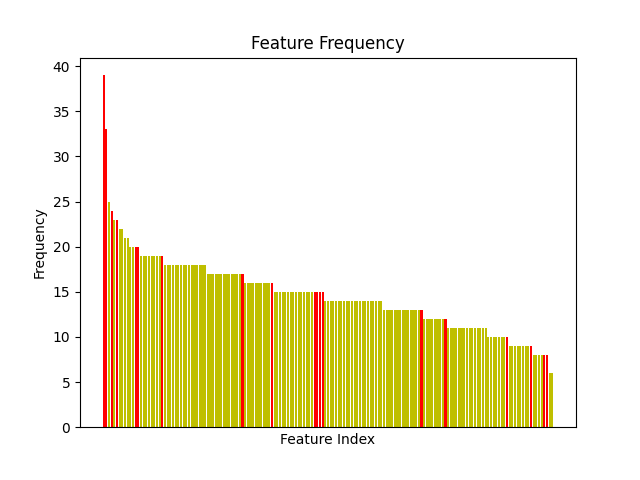
\includegraphics[scale=0.8]{./figures/Figure_all_fres.png}
  \caption{Prominence of each feature in all 40 tests sorted in descending order. Morphological features are colored red and SIFT features are colored green.}
  \label{fig:all_freq}
\end{figure}

\newpage

From the figure it is observable that two features had a higher frequency in the optimal set compared to the other features. Both of these features were morphological features. The most prominent feature was 'Solidity', which was calculated as the area of the lesion divided by the area of the lesion's convex hull. In simpler terms, the measurement gives an indication of how compact the lesion is. The second feature describes the contrast between the lesion and the surrounding skin in regard to the color red. It was calculated as the average red value of the pixels inside the lesion, divided by the average red value of the pixels outside the lesion. Thus, a value above '1' indicates that the lesion contains more of the color, while a lesser value indicates that the surrounding skin is redder than the lesion.

Concerning the difference between morphological and SIFT features table \ref{representation} show the results. 

\begin{table}[h!]
  \caption{Average number of occurrences in optimal set for ABCD and SIFT features.}
  \pgfplotstabletypeset[ col sep=comma,
    string type,
    columns={Feature Type, Number of Features, Occurence(s), Representation},
    columns/Feature Type/.style={column name=Feature Type, column type={|l|}},
    columns/Number of Features/.style={column name=Feature count, column type={l|}},
    columns/Occurence(s)/.style={column name=Occurences, column type={l|}},
    columns/Representation/.style={column name=Average Occurences, column type={l|}},
    every head row/.style={before row=\hline, after row=\hline},
    every nth row={1}{before row=\hline},
    every last row/.style={after row=\hline}
  ]{../representation.csv}
  \label{representation}
\end{table}

From table \ref{representation} it is observable that the SIFT features have more occurrences overall than the morphological features. However, if the distribution between the two types is considered, the morphological features have a higher occurrence rate per feature than the SIFT features, which can imply that the morphological features are more likely to be included in the optimal set.

\section{Determining important features for each classifier}

In this section results concerning features' importance for different classifiers are presented. To begin with the difference between the importance of SIFT and morphological features are presented in table \ref{class_sift_vs_abcd}. 

\begin{table}[h!]
  \caption{}
  \pgfplotstabletypeset[ col sep=comma,
    string type,
    columns={Classifier, Morphological Occurences, Occurences per Morphological Feature, SIFT Occurences, Occurences per SIFT Feature},
    columns/Classifier/.style={column name=Classifier, column type={|l|}},
    columns/Morphological Occurences/.style={column name=Morphological Occurences, column type={l|}},
    columns/Occurences per Morphological Feature/.style={column name=Occurences per Morphological Feature, column type={l|}},
    columns/SIFT Occurences/.style={column name=SIFT Occurences, column type={l|}},
    columns/Occurences per SIFT Feature/.style={column name=Occurences per SIFT Feature, column type={l|}},
    every head row/.style={before row=\hline, after row=\hline},
    every nth row={1}{before row=\hline},
    every last row/.style={after row=\hline}
  ]{../new_plots/csv_files/class_abcd_vs_sift.csv}
  \label{class_sift_vs_abcd}
\end{table}

The results show no particular difference between the two types of features for the KNN, NN and RF classifiers. For the SVM, however, the morphological features were more common in the feature set.

In the following subsections the results for every classifier is presented through both a figure showing the distribution of feature occurrences and a table giving more details into the results.

\subsection{K-nearest neighbors}


\begin{figure}[h!]
  \centering
  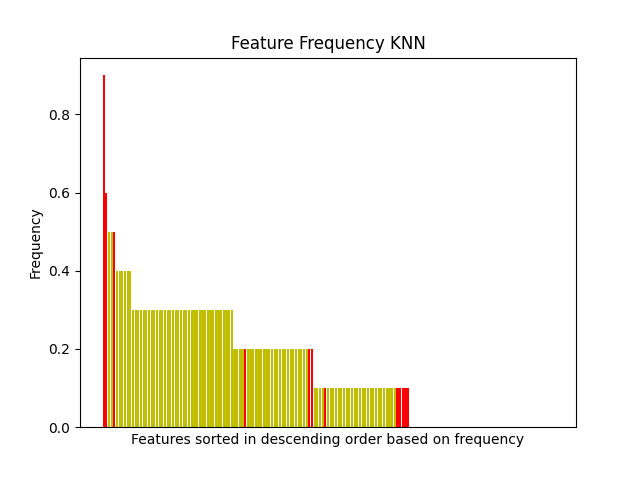
\includegraphics[scale=0.8]{figures/knn_all_freqs.png}
  \caption{Prominence of each feature in all 10 tests using KNN sorted in descending order. Morphological features are colored red and SIFT features are colored green.}
  \label{fig:freq_knn}
\end{figure}

\newpage

Figure \ref{fig:freq_knn} shows that two features had a high frequency compared the others, and amongst these two there was a gap between the most and second most prominent.

Table \ref{knn_features} presents the features which had at least five occurrences in the optimal set. Note that in total ten tests were run so five occurrences amount to a frequency of 0.5.

\begin{table}[h!]
  \caption{The features with at least 5 occurrences in the 10 tests.}
  \begin{center}
    \pgfplotstabletypeset[col sep=comma,
    string type,
    columns={Feature, Total Frequency, Frequency using SFS, Frequency using SBS},
    columns/Feature/.style={column name=Feature, column type={|l|}},
    columns/Total Frequency/.style={column name=Frequency, column type={l|}},
    columns/Frequency using SFS/.style={column name=Frequency using SFS, column type={l|}},
    columns/Frequency using SBS/.style={column name=Frequency using SBS, column type={l|}},
    every head row/.style={before row=\hline, after row=\hline},
    every nth row={1}{before row=\hline},
    every last row/.style={after row=\hline},
    row predicate/.code={% display only the first 20 rows
    \ifnum#1>4\relax
      \pgfplotstableuserowfalse
    \fi
    }
    ]{../new_plots/csv_files/knn.csv}
  \end{center}
  \label{knn_features}
\end{table}

\newpage

The results show that the feature 'Solidity' (index 151) was prominent in the KNN classifier, which is as previously mentioned a morphological feature. Likewise, the second most prominent feature was '161' which was the second most prominent feature in all tests. A final observation is that the frequency differs greatly depending on the selection method.

% Skriv om att frequencyn är väldigt olika i sfs och sbs

% New page in order to not have the tables on the same page.
\newpage

\subsection{Neural Network}

\begin{figure}[h!]
  \centering
  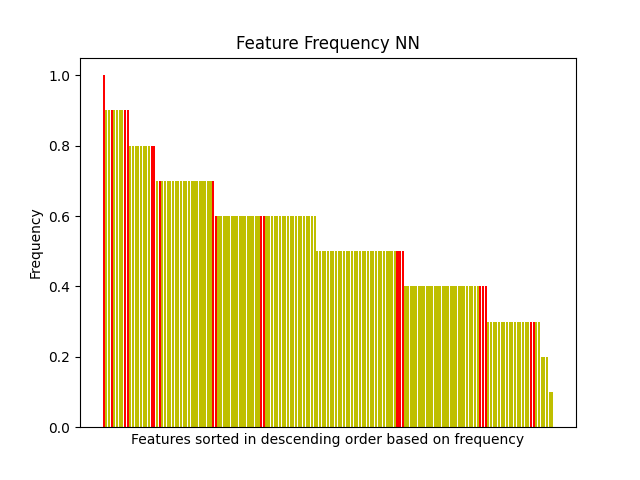
\includegraphics[scale=0.8]{figures/nn_all_freqs.png}
  \caption{Prominence of each feature in all 10 tests using NN sorted in descending order. Morphological features are colored red and SIFT features are colored green.}
  \label{fig:freq_nn}
\end{figure}

\newpage

From figure \ref{freq_nn} it is observable that the classifier had a quite even distribution overall where almost all features were present in the optimal set at least once. Furthermore the distribution between the morphological and SIFT features was slightly in the favour of the first-mentioned.  


\begin{table}[h!]
  \begin{center}
    \caption{The features with at least 9 occurrences in the 10 tests.}
    \pgfplotstabletypeset[col sep=comma,
    string type,
    columns={Feature, Total Frequency, Frequency using SFS, Frequency using SBS},
    columns/Feature/.style={column name=Feature, column type={|l|}},
    columns/Total Frequency/.style={column name=Frequency, column type={l|}},
    columns/Frequency using SFS/.style={column name=Frequency using SFS, column type={l|}},
    columns/Frequency using SBS/.style={column name=Frequency using SBS, column type={l|}},
    every head row/.style={before row=\hline, after row=\hline},
    every nth row={1}{before row=\hline},
    every last row/.style={after row=\hline},
    row predicate/.code={% display only the first 20 rows
    \ifnum#1>9\relax
      \pgfplotstableuserowfalse
    \fi
    }
    ]{../new_plots/csv_files/nn.csv}
  \end{center}
  \label{nn_features}
\end{table}

The results show that the NN classifier utilized several features where 10 features had a frequency of $0.9$ or more. Additionally, the top features were preferred by both selection methods. Lastly, the only feature that was included in the optimal set in every test was the 'Solidity' feature.

\newpage

\subsection{Random Forest}

\begin{figure}[h!]
  \centering
  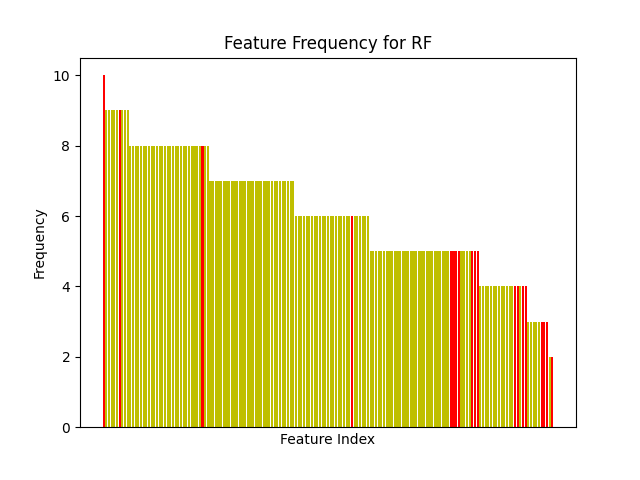
\includegraphics[scale=0.8]{figures/rf_all_freqs.png}
  \caption{Prominence of each feature in all 10 tests using RF sorted in descending order. Morphological features are colored red and SIFT features are colored green.}
  \label{fig:freqs_rf}
\end{figure}

The RF classifier preferred the SIFT features which is presented in table \ref{class_sift_vs_abcd}. This is also observable in figure \ref{fig:freqs_rf} where most morphological features have fewer occurrences compared to the SIFT features. Lastly, there was one feature that had a comparatively high frequency. The upper part of the distribution is presented in table \ref{rf_features}.

\newpage

\begin{table}[h!]
  \caption{The features with at least 9 occurences in the 10 tests.}
  \begin{center}
    \pgfplotstabletypeset[col sep=comma,
    string type,
    columns={Feature, Total Frequency, Frequency using SFS, Frequency using SBS},
    columns/Feature/.style={column name=Feature, column type={|l|}},
    columns/Total Frequency/.style={column name=Frequency, column type={l|}},
    columns/Frequency using SFS/.style={column name=Frequency using SFS, column type={l|}},
    columns/Frequency using SBS/.style={column name=Frequency using SBS, column type={l|}},
    every head row/.style={before row=\hline, after row=\hline},
    every nth row={1}{before row=\hline},
    every last row/.style={after row=\hline},
    row predicate/.code={% display only the first 20 rows
    \ifnum#1>9\relax
      \pgfplotstableuserowfalse
    \fi
    }
    ]{../new_plots/csv_files/rf.csv}
  \end{center}
  \label{rf_features}
\end{table}

Random forest, similar to Neural Network, utilized several features to a high degree. The most prominent feature was 151, which is the morphological feature 'Solidity'. Apart from this feature, the only other morphological feature with a frequency of $0.9$ was feature 166 which, like feature 160, describes a difference between the lesion and the surrounding skin in terms of the color red.


\newpage

\subsection{Support Vector Machine}

\begin{figure}[h!]
  \centering
  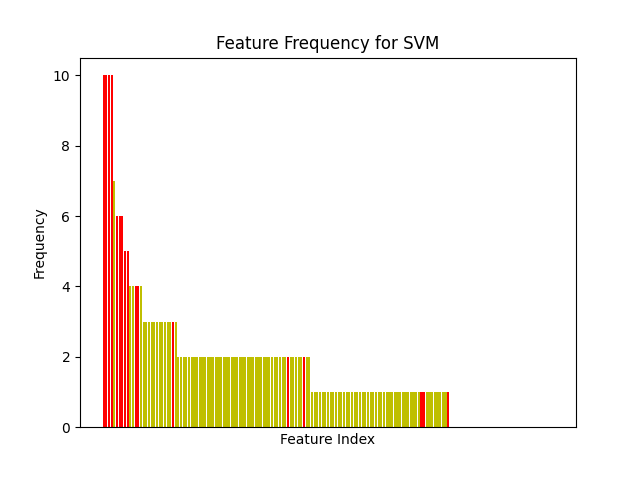
\includegraphics[scale=0.8]{figures/svm_all_freqs.png}
  \caption{Prominence of each feature in all 10 tests using SVM sorted in descending order. Morphological features are colored red and SIFT features are colored green.}
  \label{fig:freq_svm}
\end{figure}

The SVM classifier preferred the morphological features which was shown in table \ref{class_sift_vs_abcd} which is observable in figure \ref{fig:freq_svm} where almost all of the morphological features had more occurences than the SIFT features. 

\newpage

\begin{table}[h!]
  \begin{center}
    \caption{The features with at least 5 occurrences in the 10 tests.}
    \pgfplotstabletypeset[col sep=comma,
    string type,
    columns={Feature, Total Frequency, Frequency using SFS, Frequency using SBS},
    columns/Feature/.style={column name=Feature, column type={|l|}},
    columns/Total Frequency/.style={column name=Frequency, column type={l|}},
    columns/Frequency using SFS/.style={column name=Frequency using SFS, column type={l|}},
    columns/Frequency using SBS/.style={column name=Frequency using SBS, column type={l|}},
    every head row/.style={before row=\hline, after row=\hline},
    every nth row={1}{before row=\hline},
    every last row/.style={after row=\hline},
    row predicate/.code={% display only the first 20 rows
    \ifnum#1>9\relax
      \pgfplotstableuserowfalse
    \fi
    }
    ]{../new_plots/csv_files/svm.csv}
  \end{center}
  \label{svm_features}
\end{table}

As mentioned earlier the SVM preferred morphological features. From table \ref{svm_features} it is observable that out of the features that had a frequency above $0.5$, only one was a SIFT feature.  Consequently, all except number 151 were color features from the ABCD method. Furthermore, the occurrences of features decrease quite rapidly where there are only 10 features with a frequency of $0.5$ or above. Lastly, the frequency of the features did depend on the feature selection method to a certain degree.

\newpage

\section{Difference between selection methods}
 
% TODO: Vill man plåga sig lite kan man försöka färga raderna.

\begin{table}[h!]
  \begin{center}
    \caption{The average number of features in the optimal set for the different classifiers and selection methods.}
    \pgfplotstabletypeset[col sep=comma,
    string type,
    columns={Classifier, Selection Method, Average Number of Features, Average Accuracy},
    columns/Classifier/.style={column name=Classifier, column type={|l|}},
    columns/Selection Method/.style={column name=Selection Method, column type={l|}},
    columns/Average Number of Features/.style={column name=Average Number of Features, column type={l|}},
    columns/Average Accuracy/.style={column name=Average Accuracy, column type={l|}},
    every head row/.style={before row=\hline, after row=\hline},
    every nth row={1}{before row=\hline},
    every last row/.style={after row=\hline},
    ]{../new_plots/csv_files/sel_met_avg.csv}
  \end{center}
\end{table}

The results show that the SFS method used more features on average compared to the SBS method in all cases except for the Random Forest classifier. The biggest relative difference was in the case of the KNN classifier where the SFS method used more than eight times more features than the SBS method. However, no test used all the available features to achieve the highest accuracy. The highest average accuracy was achieved by the combination of SVM and SFS.

\newpage

% TODO: Hitta på bättre namn?
\subsection{Difference in performance between selection methods}

Following are the results related to the difference in performance between the two methods for every classifier.

\subsubsection{K-Nearest Neighbors}

\begin{figure}[h!]
  \begin{center}
    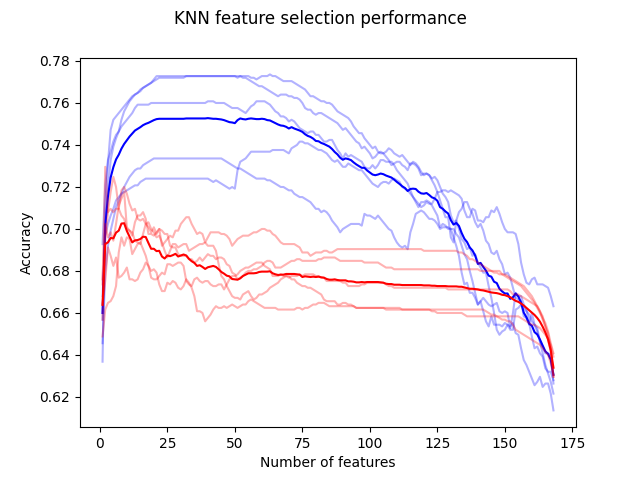
\includegraphics[scale=0.8]{../new_plots/knn_graph.png}
    \caption{Difference in performance for the KNN classifier, where each individual test is plotted with the average accuracy in bold. Tests using the SFS method are in blue while the SBS are in red. }
  \end{center}
\end{figure}

The results show that the SBS utilized less than half of the number of features compared to the SFS, where the former used around 35 features compared to the 65 features for the SFS. However, the SFS method achieved a higher accuracy than the SBS method. Another observation is a forming of plateaus where the gain in accuracy is marginal when adding features. Lastly, there was a variance in accuracy between the individual tests.

\newpage

\subsubsection{Neural Network}

\begin{figure}[h!]
  \begin{center}
    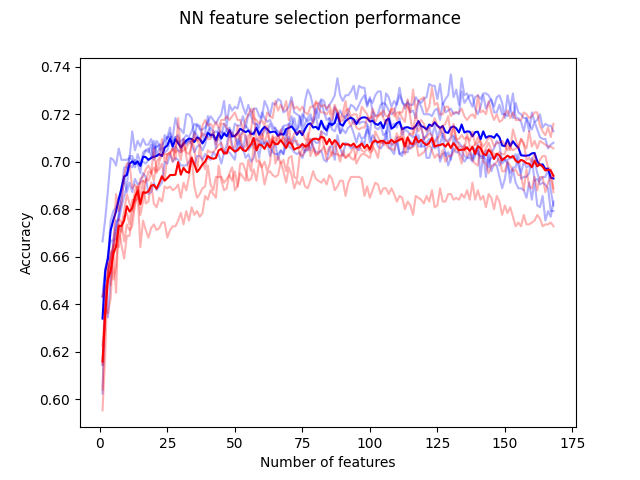
\includegraphics[scale=0.8]{../new_plots/nn_graph.png}
    \caption{Difference in performance for the NN classifier, where each individual test is plotted with the average accuracy in bold. Tests using the SFS method are in blue while the SBS are in red.}
    \label{fig:nn}  % Used to add reference in text
  \end{center}
\end{figure}

Figure \ref{fig:nn} shows that the two methods had similar results for the neural network, both in terms of performance and number of features used. None of the methods resulted in any major gains in terms of performance compared to using all features. Like in the case of the KNN there is some variance between the individual tests.

\newpage

\subsubsection{Random Forest}

\begin{figure}[h!]
  \begin{center}
    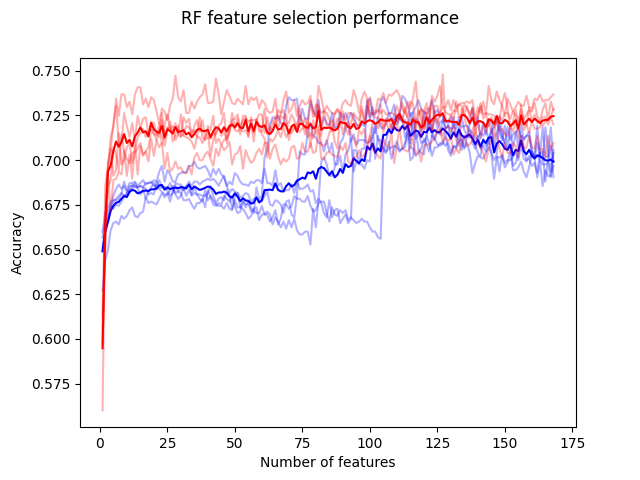
\includegraphics[scale=0.8]{../new_plots/rf_graph.png}
    \caption{Difference in performance for the RF classifier, where each individual test is plotted with the average accuracy in bold. Tests using the SFS method are in blue while the SBS are in red.}
  \end{center}
\end{figure}

Similarly to the neural network, the difference between the two methods is not vast in terms of performance. The SBS outperformed the SFS method, utilizing fewer features for a greater gain in accuracy. Secondly, like the two afformentioned classifiers, there is a variance between the different tests for both selection methods.

Lastly, in the case of the SFS method, there are spikes in all of the tests, where the performance is greatly increased when adding just a few feature. 

\newpage

\subsubsection{Support Vector Machine}

\begin{figure}[h!]
  \begin{center}
    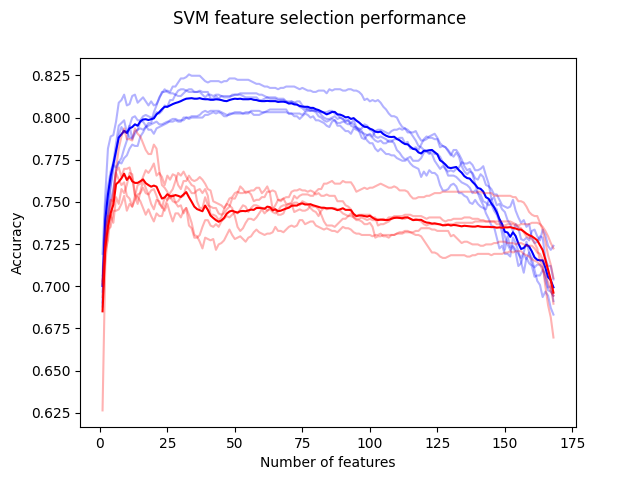
\includegraphics[scale=0.8]{../new_plots/svm_graph.png}
    \caption{Difference in performance for the SVM classifier, where each individual test is plotted with the average accuracy in bold. Tests using the SFS method are in blue while the SBS are in red.}
    \label{fig:svm}
  \end{center}
\end{figure}

Figure \ref{fig:svm} shows that they are a significant difference between the two selection methods for the SVM. The SFS method achieved an average accuracy of over 80\% while the SBS method only had one test which achieved an accuracy of over 78\%. A final observation is that like all other classifiers there is a variance for both of the selection methods.

\chapter{Discussion}

As mentioned in the result section, the morphological features were overrepresented in terms of being included in the optimal set. Similar results were achieved by \parencite{Zhang}
who compared deep features generated by a convoluted neural network against SIFT descriptors. They obtained the highest accuracy using only deep features. While mixing deep and SIFT features, the accuracy was decreased. Finally, only using SIFT features resulted in the worst observed performance. 

% Feature 151
As mentioned in the results, the most prominent feature was feature 151, which is a morphological feature. The feature measures the extent of the lesion, i.e. how many of the pixels in the image are within the lesion. This might be due to the way the tests were conducted. In the forward selection, if a feature is selected early, then it is likely to be contained in the optimal set. Thus the fact that the feature was so common might be an indicator that it was chosen early in the process. Which in turn indicates that the feature is a strong indicator on its own. However, the feature was common in both SBS and SFS, thus it might simply be an effective indicator of malignant melanoma.

% Feature 160
The second most prominent feature was feature 160, which is a color feature. As stated in the results, the feature measures the quotient of the average amount of red color within the lesion over the amount of red color in the surrounding skin. Thus, a high or low value indicates a contrast in terms of red colors between the lesion and the surrounding skin. The prominence of this feature might indicate that a contrast in terms of red color between the surrounding skin and the lesion is a common indicator of malignant melanoma. % Stödjer några källor att just färgen röd är viktigare än blå och grön?

% De stora skillnaderna mellan selection metoder
An interesting result was the difference between the two selection methods for the SVM and KNN classifiers. In both cases the SFS method achieved higher maximum accuracies while at the same time using more features than the SBS. Furthermore, the results  show that during the selection process, the SFS method had a higher average accuracy than the SBS when they utilized the same number of features. They do however converge toward the same accuracy in the beginning and end of the selection process. This indicates that there might be some hidden synergies between features where some combinations give rise to higher performance. Furthermore, this can be an indicator of that it is easier for the selection method to find these synergies when adding features rather than removing them.

Neural network and Random forest did not show any significant difference between the two selection methods. They also used more features on average in their most optimal set. Furthermore, these two models gained less in terms of performance compared to the SVM and KNN classifiers. Hence, the selection models seem to have difficulties to find effective features compared to the other classifiers.

% Att graferna och tabellerna skiljer sig åt

Furthermore, the graphs depicting the average performance of the selection methods for every classifier, and the tables presenting the average number of features used to obtain the highest accuracy for every selection method for every classifier, does not match in terms of the number of features used to obtain the highest accuracy. % Den här meningen är lite konstig. Kanske skriva om den.
For example, in the case of the SVM classifier, the SFS used on average 32,6 features and the SBS 25,4 features to obtain the highest accuracy. Meanwhile, the graph shows that the SFS obtained the highest accuracy around 24 features and the SBS around 42 features. This difference  is most likely due to the method for obtaining the results. In the former case, the accuracy of every iteration of every test was recorded. The average accuracy for every iteration was then calculated, and the graph was plotted. In the latter case, the maximum accuracy and which features constituted the optimal set was recorded. The features were then counted and the average number of features used could hence be calculated. The difference between the two test might be reduced if the number of tests performed was increased. 

% Man kan egentligen stanna tidigare än max max accuracy
Lastly, the graphs  show that for all of the methods, there is an early gain in terms of accuracy which then plateaus to then steadily decline when more and more features are added. The maximum accuracy is usually obtained towards the end of this plateau which results in a marginal gain in accuracy but a vast increase of features which increases the runtime of the algorithms. This is especially true for the KNN classifier using the SFS method, where the accuracy plateaus at around 15 features but the maximum is achieved at around 65 features. There might therefore be an interest in instead of solely measuring the accuracy, to instead introduce a two-factor system where the selection method also takes into account the increase of the feature space. Thus, the method can balance the optimal number of features dependent on both performance and runtime.


\chapter{Conclusions}

From the results, we can say that morphological features are more important than SIFT features for our classifiers' accuracy. However, there is a variance inside the morphological feature set and the best accuracy were achieved with a combination of morphological and SIFT features.

There was some variance between the difference models regarding which features were the most important. The main difference between the models were how many features were used. The SVM and KNN classifiers used fewer features than the NN and RF classifiers. 

Furthermore, the results show that the SFS method is more effective than the SBS method for the SVM and KNN classifiers. However, for the RF and NN classifiers, the two methods were equally effective.

SBS used fewer features for all models except NN, but SFS achieved better accuracy when using as many features as the SBS. % Lite märkligt men vill säga att SFS är bättre än SBS även när SBS är som bäst.

% Print the bibliography (and make it appear in the table of contents)
\printbibliography[heading=bibintoc]

% \appendix

% Tailmatter inserts the back cover page (if enabled)
\tailmatter

\end{document}
